\chapter{Architecture}
\section{OMNI Compiler}
The \clawfcomp is based on the \omni\cite{omni:website}. The \omni Project
provides a set of programs to build source-to-source translator for C/C++
and Fortran. It is jointly developed by the Programming Environment Research
Team of the RIKEN AICS and the HPCS Lab. of the University of Tsukuba both
located in Japan. The \clawfcomp is a contributor to this project. 
The \clawfcomp is using the Fortran front-end and back-end as well as the 
C back-end of the \omni. Similar transformation mechanism could be
applied without to much effort to C or C++ code by using their corresponding
fron-end. The \omni Project is actively developed as of today. Contributions or 
issues can be reported on their master repository \cite{omni:github}.

\subsection{The Fortran front-end}
The Fortran front-end is the program that parses Fortran source code and that
generates its \gls{ir}. The Fotran grammar is written in \lstinline|yacc| and 
the processing and \gls{ir} generation is written in \lstinline|C|. This program
can be called individually as shown in Listing \ref{lst:ffront}.

\begin{lstlisting}[label=lst:ffront, language=Bash, caption=Call F\_Front]
F_Front -M my_module_dir -o my_program.xml my_program.f90
\end{lstlisting}

As the \omni acts as an actual compiler, it also has a notion of module file.
When a Fortran module is parsed with the front-end, a \lstinline|.xmod| file is
generated. This file contains subroutines and function signatures and 
type definitions. This file is then needed to parse other Fortran code depending 
on the module. This mechanism allows the cross-file transformation capabilities
of the \clawfcomp.

\begin{lstlisting}[label=lst:m1, language=Fortran, caption=module\_m1.f90]
MODULE m1
  USE m2
END MODULE m1
\end{lstlisting}

\begin{lstlisting}[label=lst:m2, language=Fortran, caption=module\_m2.f90]
MODULE m2
  USE m3
END MODULE m2
\end{lstlisting}

\begin{lstlisting}[label=lst:m3, language=Fortran, caption=module\_m3.f90]
MODULE m3
END MODULE m3
\end{lstlisting}

In the simple example shown in listings \ref{lst:m1}, \ref{lst:m2} and
\ref{lst:m3}, module m1 depends on module m2 and then module m2
depends on module m3. These source files should be processed by the front-end
as shown in listing \ref{lst:ffrontdep} to respect the dependency order.

\begin{lstlisting}[label=lst:ffrontdep, language=Bash, caption=Parse module with dependencies]
F_Front -o module_m3.xml module_m3.f90      # produces m3.xmod
F_Front -M . -o module_m2.xml module_m2.f90 # uses m3.xmod and produces m2.xmod
F_Front -M . -o module_m1.xml module_m1.f90 # uses m2.xmod and produces m1.xmod
\end{lstlisting}

The \lstinline|-M| option tells the front-end where to search and store the 
module files. Several path can be given for the search but the first one will
be used to store the newly created \lstinline|.xmod| files.


\subsection{\xcodemlf}
\xcodemlf is the \gls{ir} used by the
translator in the CLAW Compiler. This \gls{ir} is based on the XML
format and is described in a specification 
document \cite{omni:xcodemlf95,omni:xcodemlf2008}. It allows to have an
high-level representation of Fortran 2008 programs.

Listing \ref{fortran1} is a simple Fortran program. Its \xcodemlf \gls{ir} is
shown in Listing \ref{xcodeml1}. A typical \xcodemlf translation unit is
composed of the followings sections:
\begin{itemize}
\item Type table with all the type definitions used in the translation unit
(Listing \ref{xcodeml1} line 6-24).
\item Global symbols table listing all the symbols at global scope in the
translation unit (Listing
\ref{xcodeml1} line 25-29).
\item Global declarations section listing the actual function and/or module
declarations in the translation unit (Listing \ref{xcodeml1} line 30-82).
\end{itemize}

\lstinputlisting
  [
    label=fortran1,
    caption=Basic Fortran program,
    language=Fortran
  ]{code/basic_fortran.f90}

\lstinputlisting
  [
    label=xcodeml1,
    caption=\xcodemlf IR,
    language=xml
  ]{code/basic_fortran.xml}

\subsection{The Fortran back-end}
The Fortran back-end is the program that decompiles \gls{ir} back to Fortran
code. It is a simple Java program that implements a visitor pattern across
the \gls{ast}. It can be called as a standalone program 
(See Listing~\ref{lst:fbackend}) or directly within the translator as it is 
done in the \clawfcomp (See Listing \ref{lst:fbackend_java}).

\begin{lstlisting}[label=lst:fbackend, language=Bash, caption=Execute the 
  Fortran back-end as a standalone]
java -cp <omni-install-path>/share/xcalablemp/om-f-back.jar:<omni-install-path>/share/xcalablemp/om-exc-tools.jar xcodeml.f.util.omx2f -l xcodeml.xml
\end{lstlisting}

\begin{lstlisting}[label=lst:fbackend_java, language=Java, 
  caption=Fortran back-end called from Java]
PrintWriter writer = 
  new PrintWriter(new BufferedWriter(new FileWriter(outputFile)));
XmToolFactory toolFactory = new XmToolFactory("F");
XmOption.setCoarrayNoUseStatement(true);
XmOption.setDebugOutput(false);
XmDecompiler decompiler = toolFactory.createDecompiler();
XmDecompilerContext context = toolFactory.createDecompilerContext();
// xcodemlDocument is the XcodeML/F DOM document to write to file
decompiler.decompile(context, xcodemlDocument, writer); 
\end{lstlisting}

The C back-end is a similar program but working on the \xcodemlc{} \gls{ir}.

\section{\clawfcomp}
The \clawfc is the program handed to the end-user. It performs all the needed
step to have a source-to-source translation of a Fortran source code. 
As shown in Figure~\ref{fig:clawfc_main_workflow}, 
it is composed by various programs under-the-hood. 
The complete workflow is devided as follows:

\begin{enumerate}
\item \textbf{FPP}: The Fortran source code is preprocessed by a standard
Fortran preprocessor.
The \lstinline|FC| environment variable is used by the CMake build system to
determine it. \textbf{FPP} is needed to have a syntactically correct Fortran
code to pass to the parser. Code with preprocessor directive is impossible 
to parse and to transform.
\item \textbf{F\_Front}: The preprocessed Fortran source code is then parsed
by the OMNI Compiler Fortran front-end to produce the input \xcodemlf \gls{ir}.
\item \textbf{CX2T}: The input \xcodemlf \gls{ir} is manipulated according to
the rules of the transformations. It produces the output \xcodeml \gls{ir}.
\item \textbf{F\_Back}: The output \xcodemlf \gls{ir} is analyzed to produce
the transformed Fortran code.
\item \textbf{C\_Back}: The output \xcodemlc \gls{ir} is analyzed to produce
the transformed C code.
\end{enumerate}

\ffront{}, \fback{}, \cback{} are part of the \omni{}, \fpp{} is provided by the
installed Fortran compiler. The \xcodemlf to \xcodeml translator \cx2x{} is
actively developed as part of the CLAW project.

\begin{figure}[!ht]
  \centering
  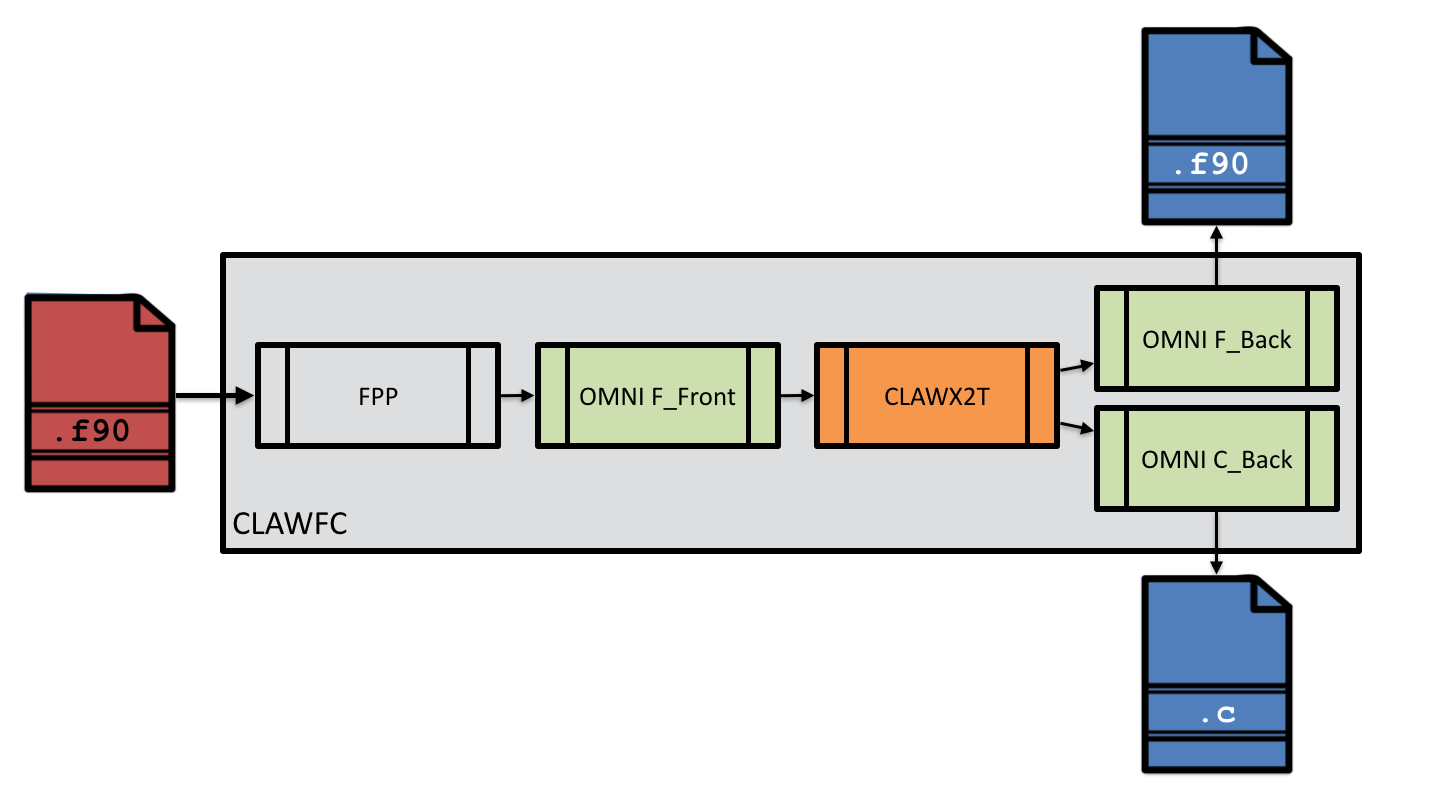
\includegraphics[
    width=0.9\textwidth
  ]{../../resources/clawfc_workflow.png} \\
  \caption{CLAW Compiler main workflow.}
  \label{fig:clawfc_main_workflow}
\end{figure}

\section{CLAW \xcodemlf to \xcodeml translator (CX2T)}
The \xcodemlf to \xcodeml translator is the intelligence behind the \clawfcomp. 
It understands the CLAW directive language, generates directive and translation 
unit transformation instances and and apply them to the to the \xcodeml
\gls{ast}.

\begin{figure}[!ht]
  \centering
  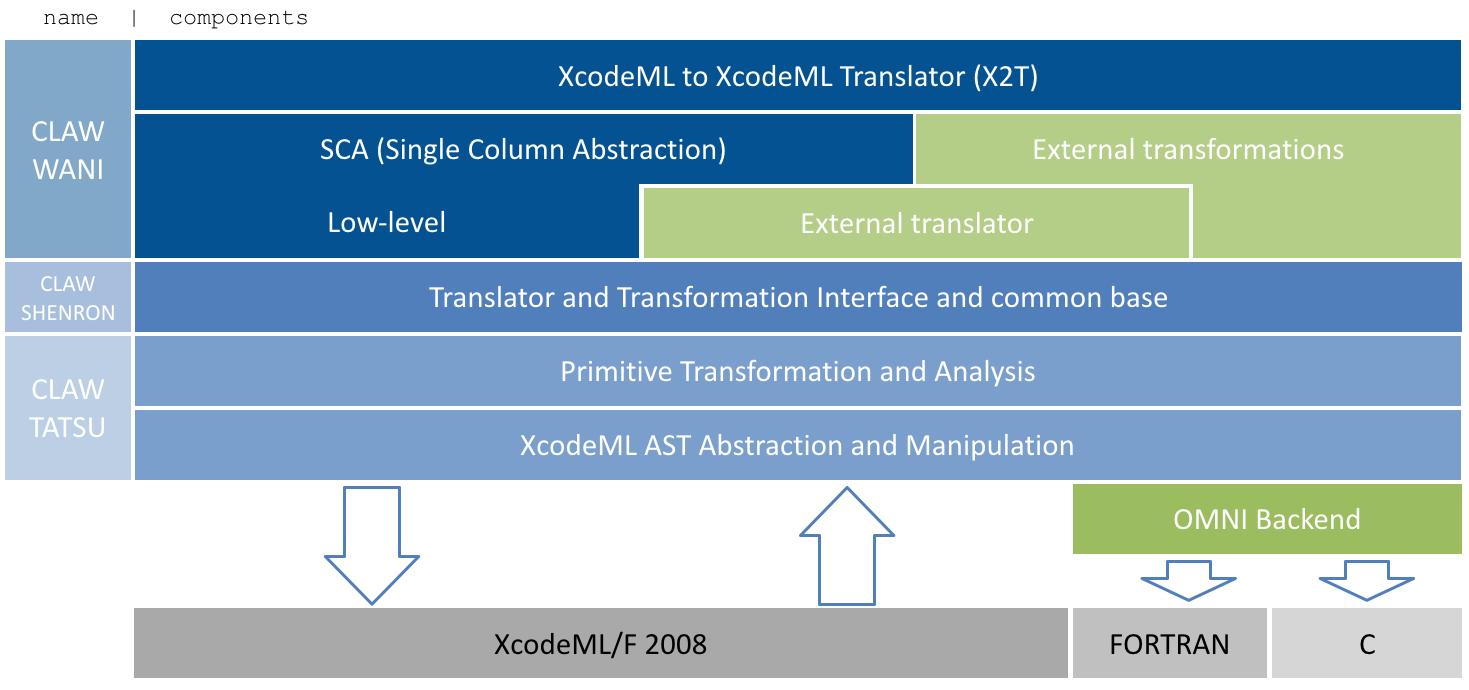
\includegraphics[width=0.9\textwidth]{../../resources/clawx2t_stack.png} \\
  \caption{CLAW \xcodemlf Translator library stack.}
  \label{fig:clawx2_stack}
\end{figure}

Figure~\ref{fig:clawx2_stack} shows the stack of libraries used in the the CLAW
\xcodemlf Translator. All blue blocks are actively developed as part of the CLAW
project. Green part are external libraries coming from the OMNI Compiler project
or from other projects using the global CLAW Compiler infrastructure.
